\documentclass[a4paper, 12pt]{article}
\usepackage[italian]{babel}
\usepackage[utf8]{inputenc}
\usepackage{graphicx}
\usepackage{float}
\frenchspacing

\title{Puzzlesolver \\ \vspace{2 mm} {\small Parte 1}}
\author{Antonio Cavestro \\ \vspace{2 mm} {\small Matricola: 1050878}}
\date{}

\begin{document}
	
  \maketitle

  \section{Abstract}

    La prima parte del progetto di Programmazione Concorrente e Distribuita prevede la realizzazione di un programma sequenziale in linguaggio Java per risolvere puzzle forniti tramite il passaggio da riga di comando del percorso del file di input. Inoltre, prevede il salvataggio della soluzione su un file il cui percorso è passato da riga di comando come secondo parametro.

    Nella seguente relazione, allegata al progetto, verranno introdotte e discusse tutte le scelte progettuali compiute per lo sviluppo del software.

  \section{Breve descrizione dell'algoritmo}

    In breve, l'algoritmo pensato per risolvere questo problema è il seguente:

    \begin{enumerate}

      \item effettuare il \emph{parsing} dei pezzi presenti nel file di input e salvarli in una struttura dati appropriata (se ne discuterà in seguito)
      \item trovare l'elemento del puzzle in alto a sinistra, riconoscibile perché l'ID del pezzo a nord e quello a ovest è uguale alla stringa \verb|VUOTO|
      \item a partire da esso, trovare la prima colonna
      \item trovare tutte le righe a partire dal primo elemento della colonna ottenuta dal punto precedente

    \end{enumerate}

	\section{Organizzazione delle classi}

    Le classi prodotte sono le seguenti:

    \begin{itemize}

      \item \verb|PuzzleSolver|
      \item \verb|unipd.cs.p3.puzzlesolver.tile.Tile|
      \item \verb|unipd.cs.p3.puzzlesolver.tile.PSTile|
      \item \verb|unipd.cs.p3.puzzlesolver.tile.TileParser|
      \item \verb|unipd.cs.p3.puzzlesolver.puzzle.Puzzle|
      \item \verb|unipd.cs.p3.puzzlesolver.puzzle.PSPuzzle|
      \item \verb|unipd.cs.p3.puzzlesolver.puzzle.PuzzleBuilder|

    \end{itemize}

    Nei prossimi paragrafi verrà discusso il motivo per cui si è stata proposta questa organizzazione e verranno descritte dettagliatamente tutte le classi ora elencate.

    \subsection{Package}

      \begin{figure}[H]

        \centering
        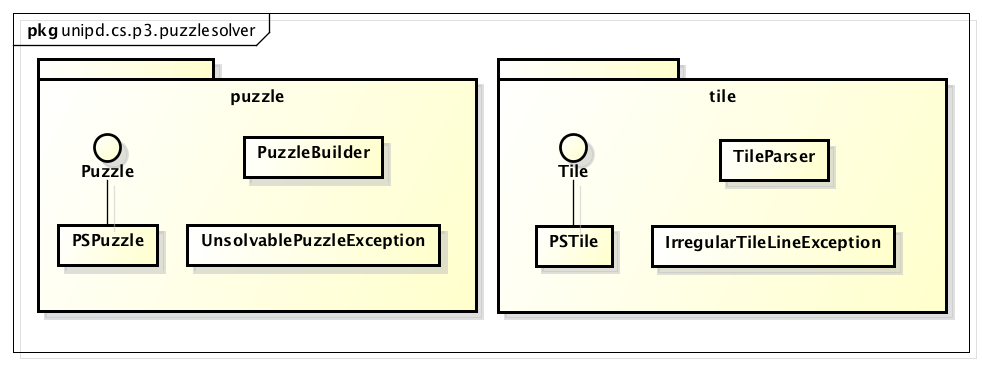
\includegraphics[scale=0.5]{uml/packages.png}
        \caption{Diagramma dei package}
        \label{uml:packages}

      \end{figure}

      La figura \ref{uml:packages} mostra l'organizzazione in package del progetto. Tutte le classi, ad eccezione di PuzzleSolver, sono contenute all'interno di un package raccoglitore chiamato \verb|unipd.cs.p3.puzzlesolver|. Quest'ultimo è a sua volta diviso in due \emph{subpackage}: \verb|tile| e \verb|package|.

      È stata preferita una suddivisione in questo senso piuttosto che creare un unico grande package in quanto quella adottata permette di separare e organizzare meglio la logica del programma.

      \begin{description}

        \item[tile] Il package \verb|tile| contiene tutto ciò che ha a che fare con i pezzi del puzzle. Descrive e contiene:

        \begin{itemize}

          \item l'interfaccia \verb|Tile|, contratto pubblico di un pezzo del puzzle
          \item un'implementazione di \verb|Tile| chiamata \verb|PSTile|
          \item la classe \verb|TileParser| che, tramite un pattern architetturale simile a \emph{Factory}, permette di ottenere una struttura dati contenente \verb|Tile| a partire da un file di testo (di discuterà di strutture dati successivamente). 

        \end{itemize}

        \item[puzzle] Il package \verb|Puzzle| contiene tutto ciò che ha a che fare con la risoluzione di un puzzle. Descrive e contiene:

        \begin{itemize}

          \item l'interfaccia \verb|Puzzle|, contratto pubblico di un puzzle \textbf{risolto}
          \item un'implementazione di \verb|Puzzle| chiamata \verb|PSPuzzle|
          \item la classe \verb|PuzzleBuilder| che risolve e costruisce un \verb|Puzzle| a partire da dei \verb|Tile|. Anch'essa, come \verb|TileParser| richiama all'uso di pattern architetturali come \emph{Factory}.

        \end{itemize}

      \end{description}

    \subsection{Package Tile}

      \subsubsection{Tile}

        \begin{figure}[H]

          \centering
          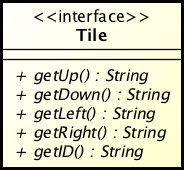
\includegraphics[scale=0.7]{uml/tile.png}
          \caption{Diagramma dell'interfaccia Tile}
          \label{uml:tile}

        \end{figure}

        \verb|Tile| è un'interfaccia che rappresenta il contratto pubblico di un pezzo del puzzle, elencato in figura ~\ref{uml:tile}. Contiene metodi per ottenere informazioni sui pezzi vicini e sul suo codice identificativo.

      \subsubsection{PSTile}

        \begin{figure}[H]

          \centering
          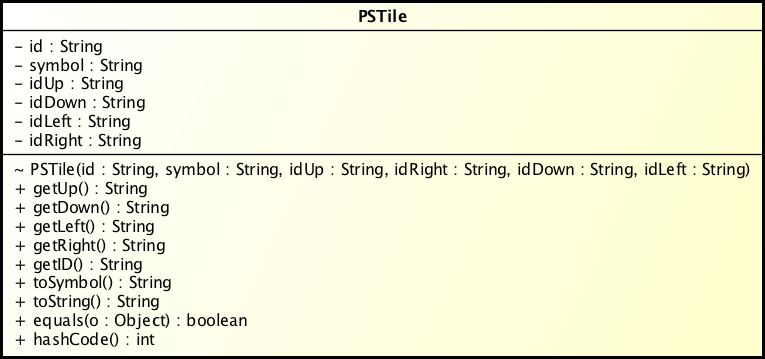
\includegraphics[scale=0.7]{uml/pstile.png}
          \caption{Diagramma della classe PSTile}
          \label{uml:pstile}

        \end{figure}

        Come si può vedere dalla figura ~\ref{uml:pstile}, la classe PSTile è una banale implementazione dell'interfaccia \verb|Tile|. 

        Da notare la ridefinizione del metodo \verb|toSymbol()| che ora restituisce una stringa come simbolo del pezzo, anziché un \verb|Object| come nella definizione dell'interfaccia. Questo è possibile in quanto \verb|String| è sottotipo di \verb|Object|.

        Il motivo per cui il metodo nell'intefaccia ritorna un oggetto generico è da attribuire alla possibilità di \verb|Tile| di essere implementata da una classe indipendente dal tipo di simbolo. Si pensi ad esempio a puzzle di immagini anziché di stringhe.

      \subsubsection{TileParser}

        \begin{figure}[H]

          \centering
          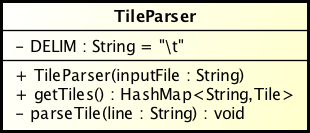
\includegraphics[scale=0.7]{uml/tileparser.png}
          \caption{Diagramma della classe TileParser}
          \label{uml:tileparser}

        \end{figure}

        La classe \verb|TileParser| ha lo scopo di ottenere una struttura dati contenente \verb|Tile| a partire da un file di testo. In particolare viene restituita una \verb|HashMap| che ha come chiave l'ID del pezzo e come valore un \verb|Tile|. 

        Questo perché \verb|HashMap|, che eredita dalla classe astratta \verb|Map|, è una struttura dati associativa, per cui è possibile ottenere un \verb|Tile| a partire dal suo solo codice identificativo, senza dover scorrere ogni volta una lista o un vettore. 

        Ciò diventa particolarmente utile quando si vuole ottenere un sequenza di \verb|Tile| consecutivi in quanto, partendo dal primo, basta ottenere l'ID di quello nella direzione desiderata e cercarlo nell'\verb|HashMap| per ottenere il successivo, fino alla fine.

        Dunque, per ottenere i \verb|Tile| si crea un oggetto della classe \verb|TileParser|, passando come parametro al costruttore il percorso del file di input. Dopodiché si chiama il metodo \verb|getTiles()| per ottenere i pezzi. 

        Il suddetto metodo non fa altro che aprire il file e ottenere un \verb|Tile| da ogni riga con il metodo privato \verb|parseTile(String)|. Questo metodo ha buone possibilità di essere reso concorrente nelle successive parti del progetto.

    \subsection{Package Puzzle}

      \subsubsection{Puzzle}

        \begin{figure}[H]

          \centering
          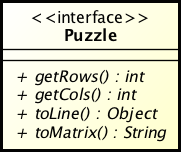
\includegraphics[scale=0.7]{uml/puzzle.png}
          \caption{Diagramma dell'interfaccia Puzzle}
          \label{uml:puzzle}

        \end{figure}

        L'interfaccia \verb|Puzzle| rappresenta il contratto pubblico di un puzzle risolto. Ha quindi i metodi per visualizzare la dimensione del puzzle e la sua forma tabellare.

      \subsubsection{PSPuzzle}

        \begin{figure}[H]

          \centering
          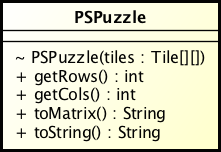
\includegraphics[scale=0.7]{uml/pspuzzle.png}
          \caption{Diagramma della classe PSPuzzle}
          \label{uml:pspuzzle}

        \end{figure}

        La classe \verb|PSPuzzle| è una banale implementazione dell'interfaccia \verb|Puzzle|. Da notare che il costruttore richiede come parametro una matrice \verb|Tile[][]|.

        Inoltre, come per la classe \verb|PSTile|, nonostante il metodo \verb|toLine| nell'interfaccia \verb|Puzzle| chieda di restituire un \verb|Object|, l'implementazione restituisce un oggetto di tipo \verb|String|.  

      \subsubsection{PuzzleBuilder}

        \begin{figure}[H]

          \centering
          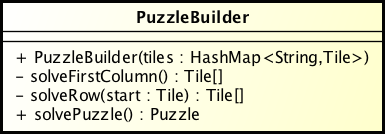
\includegraphics[scale=0.7]{uml/puzzlebuilder.png}
          \caption{Diagramma della classe PuzzleBuilder}
          \label{uml:puzzlebuilder}

        \end{figure}

        Il contratto pubblico di \verb|PuzzleBuilder| prevede che venga istanziata con una \verb|HashMap| e che, chiamando il metodo \verb|solvePuzzle()|, venga restituito un oggetto di tipo \verb|Puzzle| che rappresenta un puzzle risolto.

        Più nel dettaglio, dal punto di vista \emph{privato} della classe, il metodo \verb|solvePuzzle()| chiama innanzitutto \verb|solveFirstColumn()| che, partendo dall'elemento in alto a sinistra, trova la prima colonna del puzzle. Successivamente, per ogni elemento della colonna restituita, si chiama il metodo \verb|solveRow()| che procederà a risolvere le righe.

        In questo modo, l'unica ricerca da compiere nella struttura dati è quella del primo elemento, in alto a sinistra. Dopodiché, sfruttando le informazioni contenute in esso si procede a ricostruire la prima colonna e poi le righe.

        Si è adottato questo metodo perché è molto semplice da mettere in atto e ha buone potenzialità dal punto di vista concorrente. Con pochi aggiustamenti, il lavoro di \verb|solveRow()| potrebbe essere svolto da dei \emph{thread} che non avrebbero nemmeno bisogno di coordinarsi tra loro una volta partiti, a patto di usare strutture dati che supportano accessi e modifiche concorrenti.

    \subsection{Package di default}

      \subsubsection{PuzzleSolver}

        La classe \verb|PuzzleSolver|, contenente il metodo \verb|main|, ha innanzitutto il compito di creare un oggetto di tipo \verb|TileParser| passandogli il percorso del file di input. 

        Successivamente prende i pezzi ottenuti dal metodo \verb|getTiles()| e li riversa in un oggetto della classe \verb|PuzzleBuilder| da cui otterrà il puzzle risolto.

        Infine, deve solamente salvare il file di output come da specifica tramite le informazioni messe a disposizione dal contratto di \verb|Puzzle|.

  \section{Gestione degli errori}

    \subsection{Numero di parametri}

      All'interno della classe \verb|PuzzleSolver| viene effettuato un controllo per verificare che il programma sia stato eseguito col corretto numero di parametri. In caso contrario, viene stampato un messaggio che spiega in forma standard l'utilizzo del software dopodiché quest'ultimo si chiude.

    \subsection{Formato dei dati in input}

      Nel metodo \verb|parseLine| della classe \verb|TileParser| viene effettivamente eseguita la conversione del pezzo da stringa a oggetto di tipo \verb|Tile|. Se il numero di pezzi in cui la linea di input può essere spezzata è diverso da quello aspettato, viene lanciata un'eccezione \verb|IrregularTileLineException|. 

      Quest'ultima viene poi rilanciata dal metodo \verb|getTiles| e gestita con un messaggio d'errore all'interno del main di \verb|PuzzleSolver|.

    \subsection{Risolvibilità del puzzle}

      Il puzzle non è risolvibile se esistono riferimenti a pezzi non presenti in input o se i riferimenti stessi sono sbagliati.

      Ci sono due \emph{punti} all'interno di \verb|PuzzleBuilder| in cui è possibile controllare questo errore:

      \begin{itemize}

        \item ricerca del pezzo in alto a sinistra
        \item completamento di una riga

      \end{itemize}

      Se non si riesce a completare uno qualsiasi dei due punti precedenti, che potremmo chiamare \emph{checkpoint}, viene lanciata \verb|UnsolvablePuzzleException| gestita nel main di \verb|PuzzleSolver|.

\end{document}